\textbf{COLUNI 2020 -- Questão 29}\par\medskip Considere o gráfico a seguir, que mostra a variação aproximada de temperatura corporal de dois animais (I, II), em função da variação da temperatura ambiente:

\par

Com base no gráfico, é CORRETO afirmar que os animais I e II são, respectivamente:

% COLUNI-AUTO-FIGURES-BEGIN
\begin{figure}[htbp]
\centering
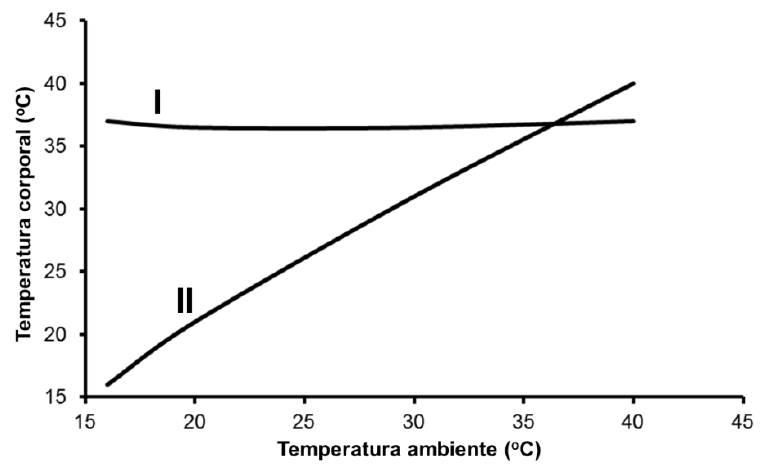
\includegraphics[width=0.95\linewidth]{static/simulados/coluni/figuras/2020/questao-29/figura-1.png}
\end{figure}
% COLUNI-AUTO-FIGURES-END
\begin{enumerate}
\item tubarão e lagartixa.
\item chimpanzé e jacaré.
\item sapo e pomba.
\item homem e galinha.\end{enumerate}
